\documentclass[twoside]{book}

% Packages required by doxygen
\usepackage{fixltx2e}
\usepackage{calc}
\usepackage{doxygen}
\usepackage{graphicx}
\usepackage[utf8]{inputenc}
\usepackage{makeidx}
\usepackage{multicol}
\usepackage{multirow}
\PassOptionsToPackage{warn}{textcomp}
\usepackage{textcomp}
\usepackage[nointegrals]{wasysym}
\usepackage[table]{xcolor}

% Font selection
\usepackage[T1]{fontenc}
\usepackage{mathptmx}
\usepackage[scaled=.90]{helvet}
\usepackage{courier}
\usepackage{amssymb}
\usepackage{sectsty}
\renewcommand{\familydefault}{\sfdefault}
\allsectionsfont{%
  \fontseries{bc}\selectfont%
  \color{darkgray}%
}
\renewcommand{\DoxyLabelFont}{%
  \fontseries{bc}\selectfont%
  \color{darkgray}%
}
\newcommand{\+}{\discretionary{\mbox{\scriptsize$\hookleftarrow$}}{}{}}

% Page & text layout
\usepackage{geometry}
\geometry{%
  a4paper,%
  top=2.5cm,%
  bottom=2.5cm,%
  left=2.5cm,%
  right=2.5cm%
}
\tolerance=750
\hfuzz=15pt
\hbadness=750
\setlength{\emergencystretch}{15pt}
\setlength{\parindent}{0cm}
\setlength{\parskip}{0.2cm}
\makeatletter
\renewcommand{\paragraph}{%
  \@startsection{paragraph}{4}{0ex}{-1.0ex}{1.0ex}{%
    \normalfont\normalsize\bfseries\SS@parafont%
  }%
}
\renewcommand{\subparagraph}{%
  \@startsection{subparagraph}{5}{0ex}{-1.0ex}{1.0ex}{%
    \normalfont\normalsize\bfseries\SS@subparafont%
  }%
}
\makeatother

% Headers & footers
\usepackage{fancyhdr}
\pagestyle{fancyplain}
\fancyhead[LE]{\fancyplain{}{\bfseries\thepage}}
\fancyhead[CE]{\fancyplain{}{}}
\fancyhead[RE]{\fancyplain{}{\bfseries\leftmark}}
\fancyhead[LO]{\fancyplain{}{\bfseries\rightmark}}
\fancyhead[CO]{\fancyplain{}{}}
\fancyhead[RO]{\fancyplain{}{\bfseries\thepage}}
\fancyfoot[LE]{\fancyplain{}{}}
\fancyfoot[CE]{\fancyplain{}{}}
\fancyfoot[RE]{\fancyplain{}{\bfseries\scriptsize Generated on Sun Nov 13 2016 20\+:16\+:33 for Lab\+C6 by Doxygen }}
\fancyfoot[LO]{\fancyplain{}{\bfseries\scriptsize Generated on Sun Nov 13 2016 20\+:16\+:33 for Lab\+C6 by Doxygen }}
\fancyfoot[CO]{\fancyplain{}{}}
\fancyfoot[RO]{\fancyplain{}{}}
\renewcommand{\footrulewidth}{0.4pt}
\renewcommand{\chaptermark}[1]{%
  \markboth{#1}{}%
}
\renewcommand{\sectionmark}[1]{%
  \markright{\thesection\ #1}%
}

% Indices & bibliography
\usepackage{natbib}
\usepackage[titles]{tocloft}
\setcounter{tocdepth}{3}
\setcounter{secnumdepth}{5}
\makeindex

% Hyperlinks (required, but should be loaded last)
\usepackage{ifpdf}
\ifpdf
  \usepackage[pdftex,pagebackref=true]{hyperref}
\else
  \usepackage[ps2pdf,pagebackref=true]{hyperref}
\fi
\hypersetup{%
  colorlinks=true,%
  linkcolor=blue,%
  citecolor=blue,%
  unicode%
}

% Custom commands
\newcommand{\clearemptydoublepage}{%
  \newpage{\pagestyle{empty}\cleardoublepage}%
}


%===== C O N T E N T S =====

\begin{document}

% Titlepage & ToC
\hypersetup{pageanchor=false,
             bookmarks=true,
             bookmarksnumbered=true,
             pdfencoding=unicode
            }
\pagenumbering{roman}
\begin{titlepage}
\vspace*{7cm}
\begin{center}%
{\Large Lab\+C6 \\[1ex]\large 1.\+0 }\\
\vspace*{1cm}
{\large Generated by Doxygen 1.8.8}\\
\vspace*{0.5cm}
{\small Sun Nov 13 2016 20:16:33}\\
\end{center}
\end{titlepage}
\clearemptydoublepage
\tableofcontents
\clearemptydoublepage
\pagenumbering{arabic}
\hypersetup{pageanchor=true}

%--- Begin generated contents ---
\chapter{Class Index}
\section{Class List}
Here are the classes, structs, unions and interfaces with brief descriptions\+:\begin{DoxyCompactList}
\item\contentsline{section}{\hyperlink{class_calculadora}{Calculadora$<$ data $>$} }{\pageref{class_calculadora}}{}
\item\contentsline{section}{\hyperlink{class_fraccion}{Fraccion} }{\pageref{class_fraccion}}{}
\item\contentsline{section}{\hyperlink{class_matriz}{Matriz} }{\pageref{class_matriz}}{}
\item\contentsline{section}{\hyperlink{class_polinomio}{Polinomio} }{\pageref{class_polinomio}}{}
\end{DoxyCompactList}

\chapter{File Index}
\section{File List}
Here is a list of all files with brief descriptions\+:\begin{DoxyCompactList}
\item\contentsline{section}{\hyperlink{_circulo_8cpp}{Circulo.\+cpp} }{\pageref{_circulo_8cpp}}{}
\item\contentsline{section}{\hyperlink{_circulo_8h}{Circulo.\+h} }{\pageref{_circulo_8h}}{}
\item\contentsline{section}{\hyperlink{_cuadrado_8cpp}{Cuadrado.\+cpp} }{\pageref{_cuadrado_8cpp}}{}
\item\contentsline{section}{\hyperlink{_cuadrado_8h}{Cuadrado.\+h} }{\pageref{_cuadrado_8h}}{}
\item\contentsline{section}{\hyperlink{_figura_8cpp}{Figura.\+cpp} }{\pageref{_figura_8cpp}}{}
\item\contentsline{section}{\hyperlink{_figura_8h}{Figura.\+h} }{\pageref{_figura_8h}}{}
\item\contentsline{section}{\hyperlink{main_8cpp}{main.\+cpp} }{\pageref{main_8cpp}}{}
\item\contentsline{section}{\hyperlink{_triangulo_8cpp}{Triangulo.\+cpp} }{\pageref{_triangulo_8cpp}}{}
\item\contentsline{section}{\hyperlink{_triangulo_8h}{Triangulo.\+h} }{\pageref{_triangulo_8h}}{}
\end{DoxyCompactList}

\chapter{Class Documentation}
\hypertarget{class_graph}{\section{Graph$<$ T $>$ Class Template Reference}
\label{class_graph}\index{Graph$<$ T $>$@{Graph$<$ T $>$}}
}


{\ttfamily \#include $<$Graph.\+h$>$}



Collaboration diagram for Graph$<$ T $>$\+:
\nopagebreak
\begin{figure}[H]
\begin{center}
\leavevmode
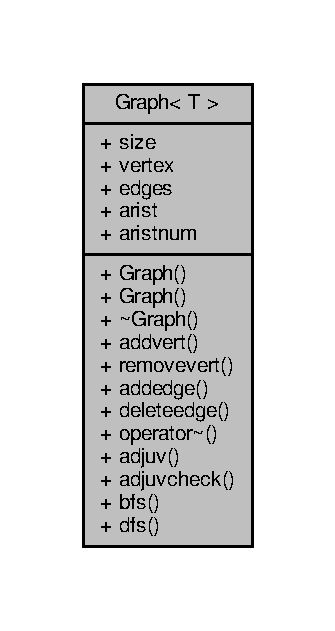
\includegraphics[width=161pt]{class_graph__coll__graph}
\end{center}
\end{figure}
\subsection*{Public Member Functions}
\begin{DoxyCompactItemize}
\item 
\hyperlink{class_graph_a8c626ac04708ae490bba05e1e713cda2}{Graph} ()
\begin{DoxyCompactList}\small\item\em Constructor de la clase grafo. \end{DoxyCompactList}\item 
\hyperlink{class_graph_a585e445e85bb506fc9b6687c15b0fbd1}{Graph} (int si, \hyperlink{class_node}{Node}$<$ T $>$ $\ast$r)
\begin{DoxyCompactList}\small\item\em Constructor sobrecargado de la clase grafo. \end{DoxyCompactList}\item 
virtual \hyperlink{class_graph_abed0ed996798032aa7dca0069a59b9d6}{$\sim$\+Graph} ()
\begin{DoxyCompactList}\small\item\em Destructor de la clase grafo. \end{DoxyCompactList}\item 
void \hyperlink{class_graph_a098e38adb75a1ede80b702ae311d3c43}{addvert} (\hyperlink{class_node}{Node}$<$ T $>$ n)
\begin{DoxyCompactList}\small\item\em Funcion que crea un vertice con tipo de dato generico. \end{DoxyCompactList}\item 
void \hyperlink{class_graph_a8051c17deea5499aff88e199eb7528a6}{removevert} (int n)
\begin{DoxyCompactList}\small\item\em Funcion que remueve un vertice. \end{DoxyCompactList}\item 
void \hyperlink{class_graph_aa0b173e1e6ba14e5290e32934a4dbc53}{addedge} (int a, int b)
\begin{DoxyCompactList}\small\item\em Funcion que cra una arista. \end{DoxyCompactList}\item 
void \hyperlink{class_graph_a43b6c33a27b9315e1559c2c611e86b47}{deleteedge} (int a, int b)
\begin{DoxyCompactList}\small\item\em Funcion que elimina una arista. \end{DoxyCompactList}\item 
void \hyperlink{class_graph_afb25283ef93b65359d82762c62dc2f27}{operator$\sim$} ()
\begin{DoxyCompactList}\small\item\em Funcion que imprime los datos del grafo. \end{DoxyCompactList}\item 
int \hyperlink{class_graph_af0776470865242ef040ecbb93226667f}{adjuv} (int n, bool $\ast$visvec)
\begin{DoxyCompactList}\small\item\em Funcion que retorna los vertices adjuntos a un vertice especifico dado. \end{DoxyCompactList}\item 
int \hyperlink{class_graph_a000c1e49d9bf261be1a4f4046a92e4cf}{adjuvcheck} (int n, bool $\ast$visvec)
\begin{DoxyCompactList}\small\item\em Funcion que verifica si un vertice posee vertices adjuntos. \end{DoxyCompactList}\item 
void \hyperlink{class_graph_a361095b62eb33806ed2df3608911c8c9}{bfs} ()
\begin{DoxyCompactList}\small\item\em Funcion que imprime el camino a seguir ara una búsqueda por ancho. \end{DoxyCompactList}\item 
void \hyperlink{class_graph_ae322c2f16b2dfd159e41ee7649899f0f}{dfs} ()
\begin{DoxyCompactList}\small\item\em Funcion que ejecuta una busqueda de profundidad en el grafo. \end{DoxyCompactList}\end{DoxyCompactItemize}
\subsection*{Public Attributes}
\begin{DoxyCompactItemize}
\item 
int \hyperlink{class_graph_a592a0bf5252e291cac9beddc3ef0dce4}{size}
\item 
\hyperlink{class_node}{Node}$<$ T $>$ $\ast$ \hyperlink{class_graph_a0f18c16458fe766ab6fff7c13b2c896e}{vertex}
\item 
bool $\ast$$\ast$ \hyperlink{class_graph_a984840929138988e3fb622fffc6b22d1}{edges}
\item 
\hyperlink{class_node}{Node}$<$ T $>$ $\ast$$\ast$ \hyperlink{class_graph_aa4d188bead6f84478f1f809c09529195}{arist}
\item 
int \hyperlink{class_graph_a5ac45f979baab5c953444780f03aca55}{aristnum}
\end{DoxyCompactItemize}


\subsection{Constructor \& Destructor Documentation}
\hypertarget{class_graph_a8c626ac04708ae490bba05e1e713cda2}{\index{Graph@{Graph}!Graph@{Graph}}
\index{Graph@{Graph}!Graph@{Graph}}
\subsubsection[{Graph}]{\setlength{\rightskip}{0pt plus 5cm}template$<$typename T$>$ {\bf Graph}$<$ T $>$\+::{\bf Graph} (
\begin{DoxyParamCaption}
{}
\end{DoxyParamCaption}
)\hspace{0.3cm}{\ttfamily [inline]}}}\label{class_graph_a8c626ac04708ae490bba05e1e713cda2}


Constructor de la clase grafo. 

\hypertarget{class_graph_a585e445e85bb506fc9b6687c15b0fbd1}{\index{Graph@{Graph}!Graph@{Graph}}
\index{Graph@{Graph}!Graph@{Graph}}
\subsubsection[{Graph}]{\setlength{\rightskip}{0pt plus 5cm}template$<$typename T$>$ {\bf Graph}$<$ T $>$\+::{\bf Graph} (
\begin{DoxyParamCaption}
\item[{int}]{si, }
\item[{{\bf Node}$<$ T $>$ $\ast$}]{r}
\end{DoxyParamCaption}
)\hspace{0.3cm}{\ttfamily [inline]}}}\label{class_graph_a585e445e85bb506fc9b6687c15b0fbd1}


Constructor sobrecargado de la clase grafo. 

\hypertarget{class_graph_abed0ed996798032aa7dca0069a59b9d6}{\index{Graph@{Graph}!````~Graph@{$\sim$\+Graph}}
\index{````~Graph@{$\sim$\+Graph}!Graph@{Graph}}
\subsubsection[{$\sim$\+Graph}]{\setlength{\rightskip}{0pt plus 5cm}template$<$typename T$>$ virtual {\bf Graph}$<$ T $>$\+::$\sim${\bf Graph} (
\begin{DoxyParamCaption}
{}
\end{DoxyParamCaption}
)\hspace{0.3cm}{\ttfamily [inline]}, {\ttfamily [virtual]}}}\label{class_graph_abed0ed996798032aa7dca0069a59b9d6}


Destructor de la clase grafo. 



\subsection{Member Function Documentation}
\hypertarget{class_graph_aa0b173e1e6ba14e5290e32934a4dbc53}{\index{Graph@{Graph}!addedge@{addedge}}
\index{addedge@{addedge}!Graph@{Graph}}
\subsubsection[{addedge}]{\setlength{\rightskip}{0pt plus 5cm}template$<$typename T$>$ void {\bf Graph}$<$ T $>$\+::addedge (
\begin{DoxyParamCaption}
\item[{int}]{a, }
\item[{int}]{b}
\end{DoxyParamCaption}
)\hspace{0.3cm}{\ttfamily [inline]}}}\label{class_graph_aa0b173e1e6ba14e5290e32934a4dbc53}


Funcion que cra una arista. 



Here is the caller graph for this function\+:\nopagebreak
\begin{figure}[H]
\begin{center}
\leavevmode
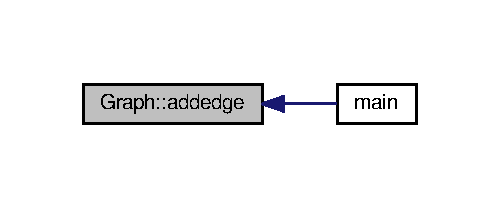
\includegraphics[width=240pt]{class_graph_aa0b173e1e6ba14e5290e32934a4dbc53_icgraph}
\end{center}
\end{figure}


\hypertarget{class_graph_a098e38adb75a1ede80b702ae311d3c43}{\index{Graph@{Graph}!addvert@{addvert}}
\index{addvert@{addvert}!Graph@{Graph}}
\subsubsection[{addvert}]{\setlength{\rightskip}{0pt plus 5cm}template$<$typename T$>$ void {\bf Graph}$<$ T $>$\+::addvert (
\begin{DoxyParamCaption}
\item[{{\bf Node}$<$ T $>$}]{n}
\end{DoxyParamCaption}
)\hspace{0.3cm}{\ttfamily [inline]}}}\label{class_graph_a098e38adb75a1ede80b702ae311d3c43}


Funcion que crea un vertice con tipo de dato generico. 



Here is the caller graph for this function\+:\nopagebreak
\begin{figure}[H]
\begin{center}
\leavevmode
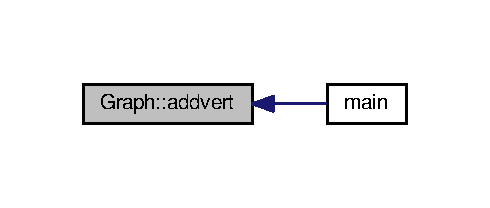
\includegraphics[width=235pt]{class_graph_a098e38adb75a1ede80b702ae311d3c43_icgraph}
\end{center}
\end{figure}


\hypertarget{class_graph_af0776470865242ef040ecbb93226667f}{\index{Graph@{Graph}!adjuv@{adjuv}}
\index{adjuv@{adjuv}!Graph@{Graph}}
\subsubsection[{adjuv}]{\setlength{\rightskip}{0pt plus 5cm}template$<$typename T$>$ int {\bf Graph}$<$ T $>$\+::adjuv (
\begin{DoxyParamCaption}
\item[{int}]{n, }
\item[{bool $\ast$}]{visvec}
\end{DoxyParamCaption}
)\hspace{0.3cm}{\ttfamily [inline]}}}\label{class_graph_af0776470865242ef040ecbb93226667f}


Funcion que retorna los vertices adjuntos a un vertice especifico dado. 

\hypertarget{class_graph_a000c1e49d9bf261be1a4f4046a92e4cf}{\index{Graph@{Graph}!adjuvcheck@{adjuvcheck}}
\index{adjuvcheck@{adjuvcheck}!Graph@{Graph}}
\subsubsection[{adjuvcheck}]{\setlength{\rightskip}{0pt plus 5cm}template$<$typename T$>$ int {\bf Graph}$<$ T $>$\+::adjuvcheck (
\begin{DoxyParamCaption}
\item[{int}]{n, }
\item[{bool $\ast$}]{visvec}
\end{DoxyParamCaption}
)\hspace{0.3cm}{\ttfamily [inline]}}}\label{class_graph_a000c1e49d9bf261be1a4f4046a92e4cf}


Funcion que verifica si un vertice posee vertices adjuntos. 

\hypertarget{class_graph_a361095b62eb33806ed2df3608911c8c9}{\index{Graph@{Graph}!bfs@{bfs}}
\index{bfs@{bfs}!Graph@{Graph}}
\subsubsection[{bfs}]{\setlength{\rightskip}{0pt plus 5cm}template$<$typename T$>$ void {\bf Graph}$<$ T $>$\+::bfs (
\begin{DoxyParamCaption}
{}
\end{DoxyParamCaption}
)\hspace{0.3cm}{\ttfamily [inline]}}}\label{class_graph_a361095b62eb33806ed2df3608911c8c9}


Funcion que imprime el camino a seguir ara una búsqueda por ancho. 



Here is the caller graph for this function\+:\nopagebreak
\begin{figure}[H]
\begin{center}
\leavevmode
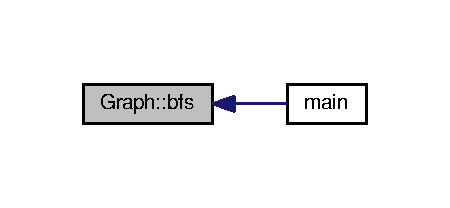
\includegraphics[width=216pt]{class_graph_a361095b62eb33806ed2df3608911c8c9_icgraph}
\end{center}
\end{figure}


\hypertarget{class_graph_a43b6c33a27b9315e1559c2c611e86b47}{\index{Graph@{Graph}!deleteedge@{deleteedge}}
\index{deleteedge@{deleteedge}!Graph@{Graph}}
\subsubsection[{deleteedge}]{\setlength{\rightskip}{0pt plus 5cm}template$<$typename T$>$ void {\bf Graph}$<$ T $>$\+::deleteedge (
\begin{DoxyParamCaption}
\item[{int}]{a, }
\item[{int}]{b}
\end{DoxyParamCaption}
)\hspace{0.3cm}{\ttfamily [inline]}}}\label{class_graph_a43b6c33a27b9315e1559c2c611e86b47}


Funcion que elimina una arista. 

\hypertarget{class_graph_ae322c2f16b2dfd159e41ee7649899f0f}{\index{Graph@{Graph}!dfs@{dfs}}
\index{dfs@{dfs}!Graph@{Graph}}
\subsubsection[{dfs}]{\setlength{\rightskip}{0pt plus 5cm}template$<$typename T$>$ void {\bf Graph}$<$ T $>$\+::dfs (
\begin{DoxyParamCaption}
{}
\end{DoxyParamCaption}
)\hspace{0.3cm}{\ttfamily [inline]}}}\label{class_graph_ae322c2f16b2dfd159e41ee7649899f0f}


Funcion que ejecuta una busqueda de profundidad en el grafo. 



Here is the caller graph for this function\+:\nopagebreak
\begin{figure}[H]
\begin{center}
\leavevmode
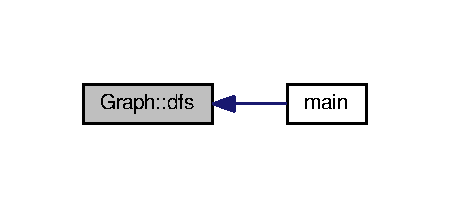
\includegraphics[width=216pt]{class_graph_ae322c2f16b2dfd159e41ee7649899f0f_icgraph}
\end{center}
\end{figure}


\hypertarget{class_graph_afb25283ef93b65359d82762c62dc2f27}{\index{Graph@{Graph}!operator````~@{operator$\sim$}}
\index{operator````~@{operator$\sim$}!Graph@{Graph}}
\subsubsection[{operator$\sim$}]{\setlength{\rightskip}{0pt plus 5cm}template$<$typename T$>$ void {\bf Graph}$<$ T $>$\+::operator$\sim$ (
\begin{DoxyParamCaption}
{}
\end{DoxyParamCaption}
)\hspace{0.3cm}{\ttfamily [inline]}}}\label{class_graph_afb25283ef93b65359d82762c62dc2f27}


Funcion que imprime los datos del grafo. 

\hypertarget{class_graph_a8051c17deea5499aff88e199eb7528a6}{\index{Graph@{Graph}!removevert@{removevert}}
\index{removevert@{removevert}!Graph@{Graph}}
\subsubsection[{removevert}]{\setlength{\rightskip}{0pt plus 5cm}template$<$typename T$>$ void {\bf Graph}$<$ T $>$\+::removevert (
\begin{DoxyParamCaption}
\item[{int}]{n}
\end{DoxyParamCaption}
)\hspace{0.3cm}{\ttfamily [inline]}}}\label{class_graph_a8051c17deea5499aff88e199eb7528a6}


Funcion que remueve un vertice. 



\subsection{Member Data Documentation}
\hypertarget{class_graph_aa4d188bead6f84478f1f809c09529195}{\index{Graph@{Graph}!arist@{arist}}
\index{arist@{arist}!Graph@{Graph}}
\subsubsection[{arist}]{\setlength{\rightskip}{0pt plus 5cm}template$<$typename T$>$ {\bf Node}$<$T$>$$\ast$$\ast$ {\bf Graph}$<$ T $>$\+::arist}}\label{class_graph_aa4d188bead6f84478f1f809c09529195}
\hypertarget{class_graph_a5ac45f979baab5c953444780f03aca55}{\index{Graph@{Graph}!aristnum@{aristnum}}
\index{aristnum@{aristnum}!Graph@{Graph}}
\subsubsection[{aristnum}]{\setlength{\rightskip}{0pt plus 5cm}template$<$typename T$>$ int {\bf Graph}$<$ T $>$\+::aristnum}}\label{class_graph_a5ac45f979baab5c953444780f03aca55}
\hypertarget{class_graph_a984840929138988e3fb622fffc6b22d1}{\index{Graph@{Graph}!edges@{edges}}
\index{edges@{edges}!Graph@{Graph}}
\subsubsection[{edges}]{\setlength{\rightskip}{0pt plus 5cm}template$<$typename T$>$ bool$\ast$$\ast$ {\bf Graph}$<$ T $>$\+::edges}}\label{class_graph_a984840929138988e3fb622fffc6b22d1}
\hypertarget{class_graph_a592a0bf5252e291cac9beddc3ef0dce4}{\index{Graph@{Graph}!size@{size}}
\index{size@{size}!Graph@{Graph}}
\subsubsection[{size}]{\setlength{\rightskip}{0pt plus 5cm}template$<$typename T$>$ int {\bf Graph}$<$ T $>$\+::size}}\label{class_graph_a592a0bf5252e291cac9beddc3ef0dce4}
\hypertarget{class_graph_a0f18c16458fe766ab6fff7c13b2c896e}{\index{Graph@{Graph}!vertex@{vertex}}
\index{vertex@{vertex}!Graph@{Graph}}
\subsubsection[{vertex}]{\setlength{\rightskip}{0pt plus 5cm}template$<$typename T$>$ {\bf Node}$<$T$>$$\ast$ {\bf Graph}$<$ T $>$\+::vertex}}\label{class_graph_a0f18c16458fe766ab6fff7c13b2c896e}


The documentation for this class was generated from the following file\+:\begin{DoxyCompactItemize}
\item 
\hyperlink{_graph_8h}{Graph.\+h}\end{DoxyCompactItemize}

\hypertarget{class_node}{\section{Node$<$ T $>$ Class Template Reference}
\label{class_node}\index{Node$<$ T $>$@{Node$<$ T $>$}}
}


{\ttfamily \#include $<$Node.\+h$>$}



Collaboration diagram for Node$<$ T $>$\+:
\nopagebreak
\begin{figure}[H]
\begin{center}
\leavevmode
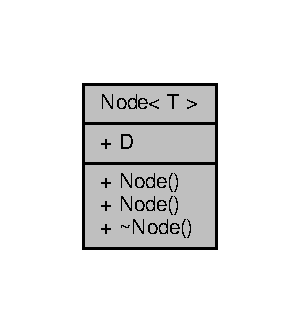
\includegraphics[width=144pt]{class_node__coll__graph}
\end{center}
\end{figure}
\subsection*{Public Member Functions}
\begin{DoxyCompactItemize}
\item 
\hyperlink{class_node_a0ac1d44cfe588be564acf25485029bd8}{Node} ()
\begin{DoxyCompactList}\small\item\em Constructor de la clase nodo. \end{DoxyCompactList}\item 
\hyperlink{class_node_a0e82c9207237470fb2438277b58f2465}{Node} (\hyperlink{class_node}{Node} $\ast$l, \hyperlink{class_node}{Node} $\ast$r, \hyperlink{class_node}{Node} $\ast$p, T $\ast$d)
\begin{DoxyCompactList}\small\item\em Constructor sobrecargado de la clase nodo. \end{DoxyCompactList}\item 
virtual \hyperlink{class_node_a9d7766f31d47a9a69927635600e34718}{$\sim$\+Node} ()
\begin{DoxyCompactList}\small\item\em Destructor de la clase nodo. \end{DoxyCompactList}\end{DoxyCompactItemize}
\subsection*{Public Attributes}
\begin{DoxyCompactItemize}
\item 
T \hyperlink{class_node_ade05a452f3fc4e823b9cdc940546e644}{D}
\end{DoxyCompactItemize}


\subsection{Constructor \& Destructor Documentation}
\hypertarget{class_node_a0ac1d44cfe588be564acf25485029bd8}{\index{Node@{Node}!Node@{Node}}
\index{Node@{Node}!Node@{Node}}
\subsubsection[{Node}]{\setlength{\rightskip}{0pt plus 5cm}template$<$typename T$>$ {\bf Node}$<$ T $>$\+::{\bf Node} (
\begin{DoxyParamCaption}
{}
\end{DoxyParamCaption}
)\hspace{0.3cm}{\ttfamily [inline]}}}\label{class_node_a0ac1d44cfe588be564acf25485029bd8}


Constructor de la clase nodo. 

\hypertarget{class_node_a0e82c9207237470fb2438277b58f2465}{\index{Node@{Node}!Node@{Node}}
\index{Node@{Node}!Node@{Node}}
\subsubsection[{Node}]{\setlength{\rightskip}{0pt plus 5cm}template$<$typename T$>$ {\bf Node}$<$ T $>$\+::{\bf Node} (
\begin{DoxyParamCaption}
\item[{{\bf Node}$<$ T $>$ $\ast$}]{l, }
\item[{{\bf Node}$<$ T $>$ $\ast$}]{r, }
\item[{{\bf Node}$<$ T $>$ $\ast$}]{p, }
\item[{T $\ast$}]{d}
\end{DoxyParamCaption}
)\hspace{0.3cm}{\ttfamily [inline]}}}\label{class_node_a0e82c9207237470fb2438277b58f2465}


Constructor sobrecargado de la clase nodo. 

\hypertarget{class_node_a9d7766f31d47a9a69927635600e34718}{\index{Node@{Node}!````~Node@{$\sim$\+Node}}
\index{````~Node@{$\sim$\+Node}!Node@{Node}}
\subsubsection[{$\sim$\+Node}]{\setlength{\rightskip}{0pt plus 5cm}template$<$typename T$>$ virtual {\bf Node}$<$ T $>$\+::$\sim${\bf Node} (
\begin{DoxyParamCaption}
{}
\end{DoxyParamCaption}
)\hspace{0.3cm}{\ttfamily [inline]}, {\ttfamily [virtual]}}}\label{class_node_a9d7766f31d47a9a69927635600e34718}


Destructor de la clase nodo. 



\subsection{Member Data Documentation}
\hypertarget{class_node_ade05a452f3fc4e823b9cdc940546e644}{\index{Node@{Node}!D@{D}}
\index{D@{D}!Node@{Node}}
\subsubsection[{D}]{\setlength{\rightskip}{0pt plus 5cm}template$<$typename T$>$ T {\bf Node}$<$ T $>$\+::D}}\label{class_node_ade05a452f3fc4e823b9cdc940546e644}


The documentation for this class was generated from the following file\+:\begin{DoxyCompactItemize}
\item 
\hyperlink{_node_8h}{Node.\+h}\end{DoxyCompactItemize}

\hypertarget{classque}{\section{que$<$ T $>$ Class Template Reference}
\label{classque}\index{que$<$ T $>$@{que$<$ T $>$}}
}


{\ttfamily \#include $<$queue.\+h$>$}



Collaboration diagram for que$<$ T $>$\+:
\nopagebreak
\begin{figure}[H]
\begin{center}
\leavevmode
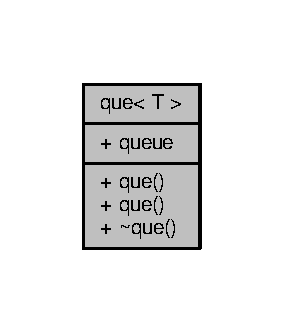
\includegraphics[width=136pt]{classque__coll__graph}
\end{center}
\end{figure}
\subsection*{Public Member Functions}
\begin{DoxyCompactItemize}
\item 
\hyperlink{classque_a238b3041fa36ddc5b657c0ba45d3e0a8}{que} ()
\item 
\hyperlink{classque_a5ec69ddb4a0ee110e9c46447af8f440d}{que} (T $\ast$qu)
\item 
virtual \hyperlink{classque_a766b884d9b0cdad120b0e2d9e6479804}{$\sim$que} ()
\end{DoxyCompactItemize}
\subsection*{Public Attributes}
\begin{DoxyCompactItemize}
\item 
T $\ast$ \hyperlink{classque_a13f6349aa25df1e706a9b8b5ef69993c}{queue}
\end{DoxyCompactItemize}


\subsection{Constructor \& Destructor Documentation}
\hypertarget{classque_a238b3041fa36ddc5b657c0ba45d3e0a8}{\index{que@{que}!que@{que}}
\index{que@{que}!que@{que}}
\subsubsection[{que}]{\setlength{\rightskip}{0pt plus 5cm}template$<$typename T $>$ {\bf que}$<$ T $>$\+::{\bf que} (
\begin{DoxyParamCaption}
{}
\end{DoxyParamCaption}
)\hspace{0.3cm}{\ttfamily [inline]}}}\label{classque_a238b3041fa36ddc5b657c0ba45d3e0a8}
\hypertarget{classque_a5ec69ddb4a0ee110e9c46447af8f440d}{\index{que@{que}!que@{que}}
\index{que@{que}!que@{que}}
\subsubsection[{que}]{\setlength{\rightskip}{0pt plus 5cm}template$<$typename T $>$ {\bf que}$<$ T $>$\+::{\bf que} (
\begin{DoxyParamCaption}
\item[{T $\ast$}]{qu}
\end{DoxyParamCaption}
)\hspace{0.3cm}{\ttfamily [inline]}}}\label{classque_a5ec69ddb4a0ee110e9c46447af8f440d}
\hypertarget{classque_a766b884d9b0cdad120b0e2d9e6479804}{\index{que@{que}!````~que@{$\sim$que}}
\index{````~que@{$\sim$que}!que@{que}}
\subsubsection[{$\sim$que}]{\setlength{\rightskip}{0pt plus 5cm}template$<$typename T $>$ virtual {\bf que}$<$ T $>$\+::$\sim${\bf que} (
\begin{DoxyParamCaption}
{}
\end{DoxyParamCaption}
)\hspace{0.3cm}{\ttfamily [inline]}, {\ttfamily [virtual]}}}\label{classque_a766b884d9b0cdad120b0e2d9e6479804}


\subsection{Member Data Documentation}
\hypertarget{classque_a13f6349aa25df1e706a9b8b5ef69993c}{\index{que@{que}!queue@{queue}}
\index{queue@{queue}!que@{que}}
\subsubsection[{queue}]{\setlength{\rightskip}{0pt plus 5cm}template$<$typename T $>$ T$\ast$ {\bf que}$<$ T $>$\+::queue}}\label{classque_a13f6349aa25df1e706a9b8b5ef69993c}


The documentation for this class was generated from the following file\+:\begin{DoxyCompactItemize}
\item 
\hyperlink{queue_8h}{queue.\+h}\end{DoxyCompactItemize}

\chapter{File Documentation}
\hypertarget{_graph_8h}{\section{Graph.\+h File Reference}
\label{_graph_8h}\index{Graph.\+h@{Graph.\+h}}
}
{\ttfamily \#include \char`\"{}Node.\+h\char`\"{}}\\*
{\ttfamily \#include $<$iostream$>$}\\*
{\ttfamily \#include $<$cstdlib$>$}\\*
{\ttfamily \#include \char`\"{}string.\+h\char`\"{}}\\*
{\ttfamily \#include $<$queue$>$}\\*
{\ttfamily \#include $<$stack$>$}\\*
Include dependency graph for Graph.\+h\+:\nopagebreak
\begin{figure}[H]
\begin{center}
\leavevmode
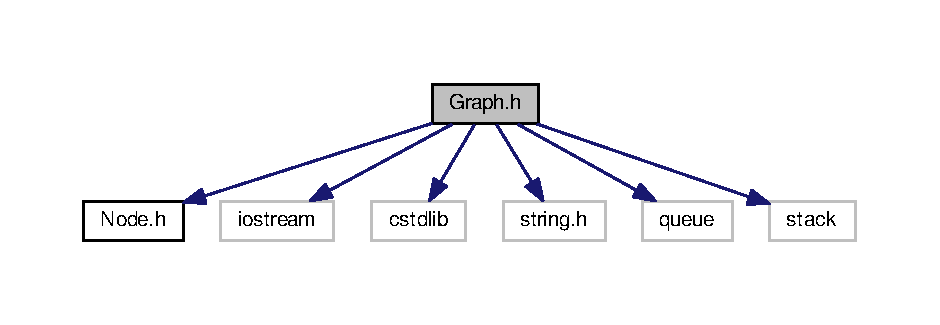
\includegraphics[width=350pt]{_graph_8h__incl}
\end{center}
\end{figure}
This graph shows which files directly or indirectly include this file\+:\nopagebreak
\begin{figure}[H]
\begin{center}
\leavevmode
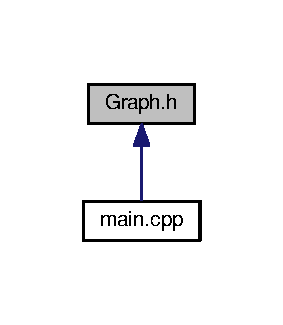
\includegraphics[width=136pt]{_graph_8h__dep__incl}
\end{center}
\end{figure}
\subsection*{Classes}
\begin{DoxyCompactItemize}
\item 
class \hyperlink{class_graph}{Graph$<$ T $>$}
\end{DoxyCompactItemize}

\hypertarget{main_8cpp}{\section{main.\+cpp File Reference}
\label{main_8cpp}\index{main.\+cpp@{main.\+cpp}}
}
{\ttfamily \#include $<$cstdlib$>$}\\*
{\ttfamily \#include \char`\"{}Node.\+h\char`\"{}}\\*
{\ttfamily \#include \char`\"{}Graph.\+h\char`\"{}}\\*
{\ttfamily \#include $<$queue$>$}\\*
Include dependency graph for main.\+cpp\+:\nopagebreak
\begin{figure}[H]
\begin{center}
\leavevmode
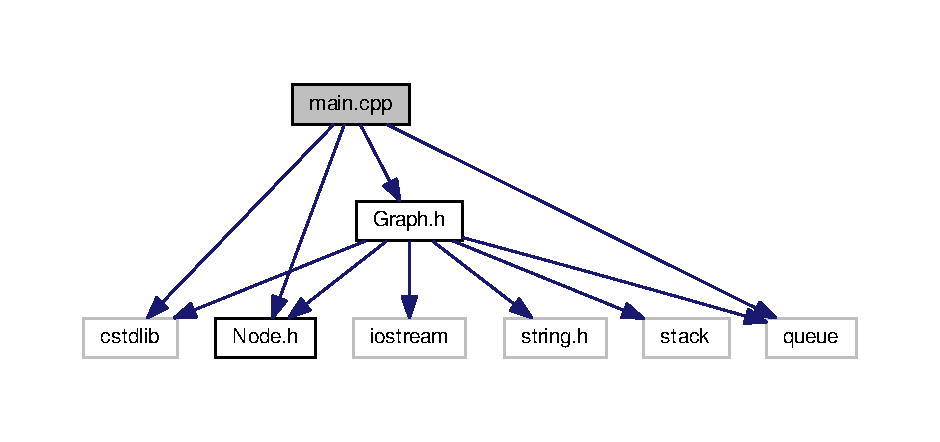
\includegraphics[width=350pt]{main_8cpp__incl}
\end{center}
\end{figure}
\subsection*{Macros}
\begin{DoxyCompactItemize}
\item 
\#define \hyperlink{main_8cpp_a4fc34b120ed3bd1120c1eb36abbcd6af}{N\+L}~cout $<$$<$ endl;
\item 
\#define \hyperlink{main_8cpp_aecd69d9a67487cc45c38eb184c50538a}{S\+P}~\char`\"{} \char`\"{}
\end{DoxyCompactItemize}
\subsection*{Functions}
\begin{DoxyCompactItemize}
\item 
int \hyperlink{main_8cpp_a3c04138a5bfe5d72780bb7e82a18e627}{main} (int argc, char $\ast$$\ast$argv)
\end{DoxyCompactItemize}


\subsection{Macro Definition Documentation}
\hypertarget{main_8cpp_a4fc34b120ed3bd1120c1eb36abbcd6af}{\index{main.\+cpp@{main.\+cpp}!N\+L@{N\+L}}
\index{N\+L@{N\+L}!main.\+cpp@{main.\+cpp}}
\subsubsection[{N\+L}]{\setlength{\rightskip}{0pt plus 5cm}\#define N\+L~cout $<$$<$ endl;}}\label{main_8cpp_a4fc34b120ed3bd1120c1eb36abbcd6af}
\hypertarget{main_8cpp_aecd69d9a67487cc45c38eb184c50538a}{\index{main.\+cpp@{main.\+cpp}!S\+P@{S\+P}}
\index{S\+P@{S\+P}!main.\+cpp@{main.\+cpp}}
\subsubsection[{S\+P}]{\setlength{\rightskip}{0pt plus 5cm}\#define S\+P~\char`\"{} \char`\"{}}}\label{main_8cpp_aecd69d9a67487cc45c38eb184c50538a}


\subsection{Function Documentation}
\hypertarget{main_8cpp_a3c04138a5bfe5d72780bb7e82a18e627}{\index{main.\+cpp@{main.\+cpp}!main@{main}}
\index{main@{main}!main.\+cpp@{main.\+cpp}}
\subsubsection[{main}]{\setlength{\rightskip}{0pt plus 5cm}int main (
\begin{DoxyParamCaption}
\item[{int}]{argc, }
\item[{char $\ast$$\ast$}]{argv}
\end{DoxyParamCaption}
)}}\label{main_8cpp_a3c04138a5bfe5d72780bb7e82a18e627}


Here is the call graph for this function\+:\nopagebreak
\begin{figure}[H]
\begin{center}
\leavevmode
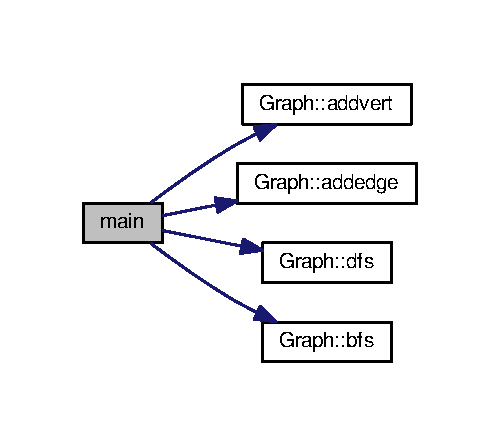
\includegraphics[width=240pt]{main_8cpp_a3c04138a5bfe5d72780bb7e82a18e627_cgraph}
\end{center}
\end{figure}



\hypertarget{_node_8h}{\section{Node.\+h File Reference}
\label{_node_8h}\index{Node.\+h@{Node.\+h}}
}
This graph shows which files directly or indirectly include this file\+:\nopagebreak
\begin{figure}[H]
\begin{center}
\leavevmode
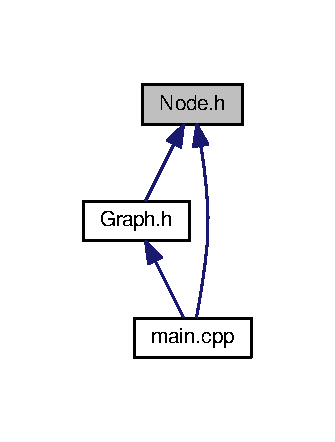
\includegraphics[width=161pt]{_node_8h__dep__incl}
\end{center}
\end{figure}
\subsection*{Classes}
\begin{DoxyCompactItemize}
\item 
class \hyperlink{class_node}{Node$<$ T $>$}
\end{DoxyCompactItemize}

\hypertarget{queue_8h}{\section{queue.\+h File Reference}
\label{queue_8h}\index{queue.\+h@{queue.\+h}}
}
\subsection*{Classes}
\begin{DoxyCompactItemize}
\item 
class \hyperlink{classque}{que$<$ T $>$}
\end{DoxyCompactItemize}

%--- End generated contents ---

% Index
\newpage
\phantomsection
\addcontentsline{toc}{chapter}{Index}
\printindex

\end{document}
